\documentclass{standalone}
\usepackage{pgfplots}
\usetikzlibrary{arrows.meta}
\pgfplotsset{compat=1.17}

\begin{document}

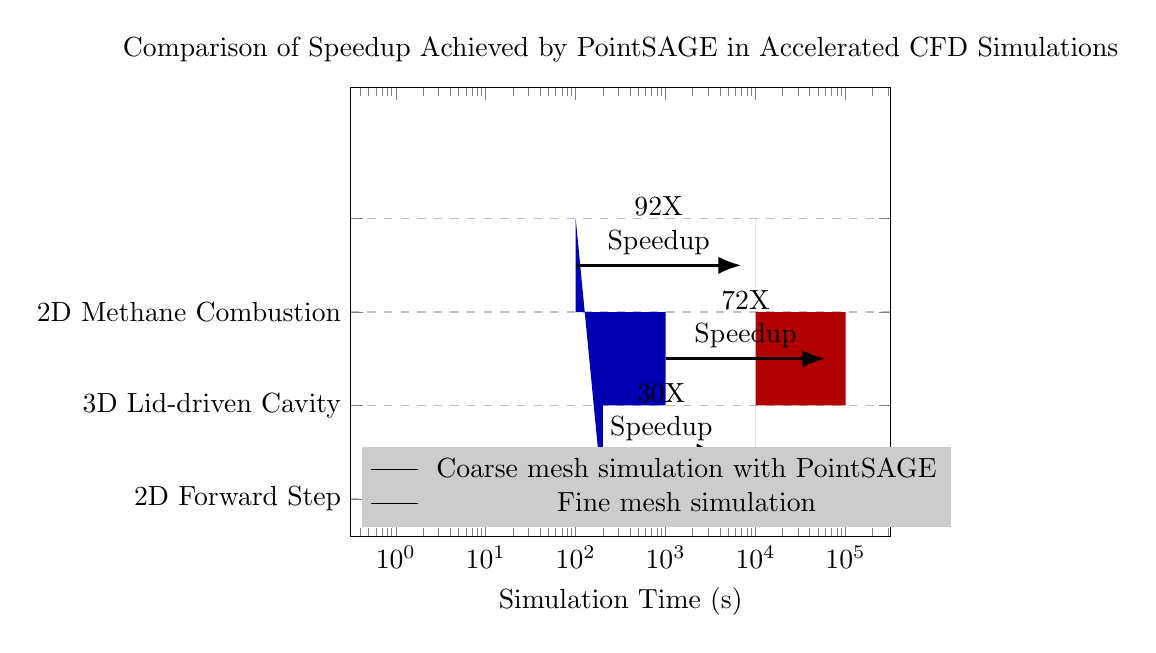
\begin{tikzpicture}
    \begin{axis}[
        title={Comparison of Speedup Achieved by PointSAGE in Accelerated CFD Simulations},
        xmode=log,
        xmin=1, xmax=1e5,
        ymin=0, ymax=4,
        ytick=data,
        yticklabels={
            2D Forward Step,
            3D Lid-driven Cavity,
            2D Methane Combustion
        },
        xlabel={Simulation Time (s)},
        xticklabel style={/pgf/number format/fixed},
        ymajorgrids=true,
        grid style=dashed,
        enlarge x limits=0.1,
        enlarge y limits=0.1,
        bar width=8pt,
        legend columns=1,
        legend style={
            at={(0.02,0.02)},
            anchor=south west,
            draw=none,
            fill=white!80!black,
            column sep=1ex
        }
    ]

    % Red bars (Fine mesh simulation)
    \addplot [draw=none, fill=red!70!black] coordinates {
        (1e4, 0) (1e4, 1)   % 2D Forward Step
        (1e5, 1) (1e5, 2)   % 3D Lid-driven Cavity
        (1e4, 2) (1e4, 3)   % 2D Methane Combustion
    };

    % Blue bars (Coarse mesh simulation + PointSAGE)
    \addplot [draw=none, fill=blue!70!black] coordinates {
        (2e2, 0) (2e2, 1)   % 2D Forward Step
        (1e3, 1) (1e3, 2)   % 3D Lid-driven Cavity
        (1e2, 2) (1e2, 3)   % 2D Methane Combustion
    };

    % Arrows and annotations
    \draw[-Latex, very thick] (axis cs:2e2,0.5) -- ++(20,0) node[midway, above, align=center] {30X \\ Speedup};
    \draw[-Latex, very thick] (axis cs:1e3,1.5) -- ++(60,0) node[midway, above, align=center] {72X \\ Speedup};
    \draw[-Latex, very thick] (axis cs:1e2,2.5) -- ++(70,0) node[midway, above, align=center] {92X \\ Speedup};

    % Legend
    \legend{
        Coarse mesh simulation with PointSAGE,
        Fine mesh simulation
    };

    \end{axis}
\end{tikzpicture}

\end{document}